\documentclass[../main.tex]{subfiles}
\graphicspath{{\subfix{../images/}}}
\begin{document}
\subsection*{Answers - Trig substitutions for integration (page \pageref{Trig substitution})}
\begin{enumerate}
    \item 
    \(\int \sqrt{1-x^2}\,dx\)
    \begin{figure}[h]
        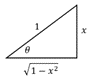
\includegraphics{images/trigsuba1.png}
    \end{figure}

    \(\sin{\theta}=x\\
    dx=\cos{\theta}\, d\theta\)
    
    Substituting into the integral:

    \(\int \sqrt{1-\sin^2{\theta}}\cos{\theta}\,d\theta\)

    \(\int \sqrt{\cos^2{\theta}}\cos{\theta}\,d\theta\)

    \(\int \cos^2{\theta} \,d\theta\)

    Using the identity \(\cos{(2\theta)}=2\cos^2{(\theta)}-1\), we know that \(\cos^2{theta}=\frac{1}{2}(\cos{(2\theta)}+1)\)

    \(\frac{1}{2}\int (\cos{(2\theta)}+1)\,d\theta=\frac{1}{2}(\frac{1}{2}\sin{(2\theta)}+\theta)+c\)

    \(=\frac{1}{4}\sin{(2\theta)}+\frac{\theta}{2}+c\)

    Use the identity \(sin{(2\theta)}=2\sin{\theta}\cos{\theta}\) to rewrite:

    \(=\frac{1}{2}\sin{\theta}\cos{\theta}+\frac{\theta}{2}+c\)

    Rewriting in terms of \(x\):

    \(\int \sqrt{1-x^2}\,dx=\frac{x\sqrt{1-x^2}}{2}+\frac{\sin^{-1}{x}}{2}+c\)

    \item 
    \(\int \sqrt{4-9x^2}\,dx\)
    \begin{figure}[h]
        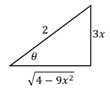
\includegraphics{images/trigsuba2.png}
    \end{figure}

    \(\sin{\theta}=\frac{3x}{2}\\
    x=\frac{2}{3}\sin{\theta}\\
    dx=\frac{2}{3}\cos{\theta}\,d\theta\)

    Substituting into the integral:

    \(\int \sqrt{4-9(\frac{2}{3}\sin{\theta})^2} \times \frac{2}{3}\cos{\theta}\,d\theta\)

    \(\frac{2}{3}\int \sqrt{4-4sin^2{\theta}}\cos{\theta}\,d\theta\)
    
    \(\frac{2}{3}\sqrt{4cos^2{\theta}}\cos{\theta}\,d\theta\)

    \(\frac{2}{3}\int 2\cos^2{\theta}\,d\theta=\frac{4}{3}\int \cos^2{\theta}\,d\theta\)

    Using the identity \(\cos{2\theta}=2\cos^2{\theta}-1\), we know \(\cos^2{\theta}=\frac{1}{2}(\cos{2\theta}+1)\)

    \(\frac{4}{3}\int \cos^2{\theta}\,d\theta=\frac{2}{3}\int (\cos{2\theta}+1)\,d\theta\)

    \(=\frac{2}{3}(\frac{1}{2}\sin{2\theta}+\theta)+c\)

    Using the sine double-angle identity:

    \(\frac{2}{3}\sin{\theta}\cos{\theta}+\frac{2}{3}\theta+c\)

    Rewriting in terms of \(x\) by using the original triangle:

    \(\int \sqrt{4-9x^2}\,dx=\frac{2}{3}\times \frac{3x}{2}\times \frac{\sqrt{4-9x^2}}{2}+\frac{2}{3}\sin^{-1}{(\frac{3x}{2})}+c\)

    \(=\frac{x\sqrt{4-9x^2}}{2}+\frac{2}{3}\sin^{-1}{(\frac{3x}{2})}+c\)

    \item 
    \(\int \sqrt{1-7x^2}\,dx\)
    \begin{figure}[h]
        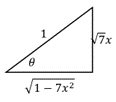
\includegraphics{images/trigsuba3.png}
    \end{figure}

    \(\sin{\theta}=\sqrt{7}x\\
    x=\frac\sin{\theta}{\sqrt{7}}\\
    dx=\frac{1}{\sqrt{7}}\cos{\theta}\,d\theta\)

    Substituting into the integral:

    \(\int \sqrt{1-7(\frac{\sin{\theta}}{\sqrt{7}})^2}\frac{1}{\sqrt{7}}\cos{\theta}\,d\theta\)

    \(\int \sqrt{1-\sin^2{\theta}}\frac{1}{\sqrt{7}}\cos{\theta}\,d\theta\)

    \(\int \sqrt{\cos^2{\theta}}\frac{1}{\sqrt{7}}\cos{\theta}\,d\theta\)

    \(\frac{1}{\sqrt{7}}\int \cos^2{\theta}\,d\theta\)
    
    Using the identity \(\cos{2\theta}=2\cos^2{\theta}-1\), we know \(\cos^2{\theta}=\frac{1}{2}(\cos{2\theta}+1)\)

    \(\frac{1}{\sqrt{7}}\int \frac{1}{2}(\cos{2\theta}+1)\,d\theta\)

    \(\frac{1}{2\sqrt{7}}\int (\cos{2\theta}+1)\,d\theta\)
    
    \(=\frac{1}{2\sqrt{7}}(\frac{1}{2}\sin{2\theta}+\theta)+c\)

    \(=\frac{1}{4\sqrt{7}}\sin{2\theta}+\frac{1}{2\sqrt{7}}\theta+c\)

    Use the sine double-angle identity:

    \(=\frac{1}{4\sqrt{7}}2\sin{\theta}\cos{\theta}+\frac{1}{2\sqrt{7}}\theta+c\)

    \(=\frac{1}{2\sqrt{7}}\sin{\theta}\cos{\theta}+\frac{1}{2\sqrt{7}}\theta+c\)

    Using the original triangle to rewrite in terms of \(x\):

    \(\int \sqrt{1-7x^2}\,dx=\frac{1}{2\sqrt{7}}\times \sqrt{7}x\sqrt{1-7x^2}+\frac{\sin^{-1}{\sqrt{7}x}}{2\sqrt{7}}+c\)

    \(\int \sqrt{1-7x^2}\,dx=\frac{x\sqrt{1-7x^2}}{2}+\frac{\sin^{-1}{\sqrt{7}x}}{2\sqrt{7}}+c\)
    
    \item 
    \(\int \frac{\sqrt{x^2+16}}{x^4}\,dx\)
    \begin{figure}[h]
        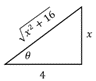
\includegraphics{images/trigsuba4.png}
    \end{figure}

    \(\tan{\theta}=\frac{x}{4}\\
    x=4\tan{\theta}\\
    dx=4\sec^2{\theta}\,d\theta\)

    Substitute into the integral:

    \(\int \frac{\sqrt{16\tan^2{\theta}+16}}{256\tan^4{\theta}}\,d\theta\)

    We can simplify \(\sqrt{16\tan^2{\theta}+16}=\sqrt{16(\tan^2{\theta}+1)}=\sqrt{16\sec^2{\theta}}=4\sec{\theta}\)
    
    \(\int \frac{16\sec^3{\theta}}{256\tan^4{\theta}}\,d\theta=\frac{1}{16}\int \frac{\sec^3{\theta}}{\tan^4{\theta}}\,d\theta\)

    \(=\frac{1}{16}\int \frac{1}{\cos^3{\theta}}\times \frac{\cos^4{\theta}}{\sin^4{\theta}}\,d\theta=\frac{1}{16}\int \frac{\cos{\theta}}{\sin^4{\theta}}\,d\theta\)

    Integrate with substitution, \(u=\sin{\theta}, du=\cos{\theta}\,d\theta\)

    \(=\frac{1}{16}\int \frac{1}{u^4}\,du\)

    \(=\frac{1}{16}\times -\frac{1}{3u^3}+c\)

    \(=\frac{1}{48\sin^3{\theta}}+c\)

    Rewriting in terms of x, where \(\sin{\theta}=\frac{x}{\sqrt{x^2+16}}\)

    \(\int \frac{\sqrt{x^2+16}}{x^4}\,dx=-\frac{(x^2+16)^\frac{3}{2}}{48x^3}+c\)

    \item 
    \(\int \frac{2}{x^4\sqrt{x^2-25}}\,dx\)
    \begin{figure}[h]
        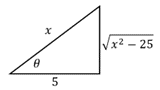
\includegraphics{images/trigsuba5.png}
    \end{figure}

    \(\cos{\theta}=\frac{5}{x}\\
    x=5\sec{\theta}\\
    dx=5\sec{\theta}\tan{\theta}\,d\theta\)

    Substitute into the integral:

    \(2\int \frac{5\sec{\theta}\tan{\theta}}{625\sec^4{\theta}\sqrt{25\sec^2{\theta}-25}}\,d\theta\)

    We know that \(\sqrt{25\sec^2{\theta}-25}=\sqrt{25(\sec^2{\theta}-1)}=\sqrt{25\tan^2{\theta}}=5\tan{\theta}\)

    \(2\int \frac{5\sec{\theta}\tan{\theta}}{625\sec^4{\theta}\times 5\tan{\theta}}\,d\theta\)

    \(=\frac{2}{625}\int \frac{1}{\sec^3{\theta}}\,d\theta=\frac{2}{625}\int \cos^3{\theta}\,d\theta\)

    To integrate we now need to split the \(\cos^3{\theta}\) into \(\cos{\theta}\cos^2{\theta}=\cos{\theta}(1-\sin^2{\theta})\), giving us:

    \(\frac{2}{625}\int \cos{\theta}-\sin^2{\theta}\cos{\theta}\,d\theta\)

    \(=\frac{2}{625}(\sin{\theta}-\frac{1}{3}\sin^3{\theta})+c=\frac{2\sin{\theta}}{625}-\frac{2\sin^3{\theta}}{1875}+c\)

    Rewriting back in terms of x, where \(\sin{\theta}=\frac{\sqrt{x^2-25}}{x}\):

    \(\int \frac{2}{x^4\sqrt{x^2-25}}\,dx=\frac{2\sqrt{x^2-25}}{625x}-\frac{2(x^2-25)^\frac{3}{2}}{1875x^3}+c\)

    \item 
    \(\int x^3(3x^2-4)^{\frac{5}{2}}\,dx\)
    \begin{figure}[h]
        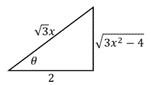
\includegraphics{images/trigsuba6.png}
    \end{figure}

    \(\cos{\theta}=\frac{2}{\sqrt{3}x}\\
    x=\frac{2\sec{\theta}}{\sqrt{3}}\\
    dx=\frac{2}{\sqrt{3}\sec{\theta}\tan{\theta}}\)

    Substitute into the integral:

    \((\frac{2}{\sqrt{3}})^3\int \sec^3{\theta}(3\times \frac{4}{3}\sec^2{\theta}-4)^{\frac{5}{2}}\times \frac{2}{\sqrt{3}}\sec{\theta}\tan{\theta}\,d\theta\)

    \(\frac{16}{9}\int \sec^4{\theta}\tan{\theta}(4\tan^2{\theta})^{\frac{5}{2}}\,d\theta\)

    \(\frac{16}{9}\int \sec^4{\theta}\tan{\theta}\times 32\tan^5{\theta}\,d\theta\)

    \(\frac{512}{9}\int \sec^4{\theta}\tan^6{\theta}\,d\theta\)

    Making a substitution of \(u=\tan{\theta}, du=\sec^2{\theta}\) (and remembering that \(\sec^2{\theta}=\tan^2{\theta}+1)\)

    \(\frac{512}{9}\int \sec^2{\theta}\tan^6{\theta}\sec^2{\theta}\,d\theta\) becomes \(\frac{512}{9}\int (u^2+1)u^6\,du\)

    \(\frac{512}{9}\int (u^8+u^6\,du)=\frac{512}{9}(\frac{u^9}{9}+\frac{u^7}{7})+c\)

    Substituting back in:

    \(\frac{512}{9}(\frac{\tan^9{\theta}}{9}+\frac{\tan^7{\theta}}{7})+c\)

    And finally, rewriting in terms of $x$:

    \(\frac{512}{9}(\frac{(\frac{\sqrt{3x^2-4}}{2})^9}{9}+\frac{(\frac{\sqrt{3x^2-4}}{2})^7}{7})+c\)

    \(=\frac{512}{81}\frac{(3x^2-4)^\frac{9}{2}}{512}+\frac{512}{63}\frac{(3x^2-4)^\frac{7}{2}}{128}+c\)

    \(=\frac{(3x^2-4)^\frac{9}{2}}{81}+\frac{4(3x^2-4)^\frac{7}{2}}{63}+c\)

    \item 
    \(\int x^3\sqrt{4-9x^2}\,dx\)

    \begin{figure}[h]
        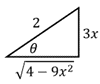
\includegraphics{images/trigsuba7.png}
    \end{figure}

    \(\sin{\theta}=\frac{3x}{2}\\
    x=\frac{2}{3}\sin{\theta}\\
    dx=\frac{2}{3}\cos{\theta}\)

    \(\int (\frac{2}{3}\sin{\theta})^3\sqrt{4-9(\frac{4}{9}\sin^2{\theta})}\frac{2}{3}\cos{\theta}\,d\theta\)

    \(\int \frac{8}{27}\sin^3{\theta}\times 2\cos{\theta}\times \frac{2}{3}\cos{\theta}\,d\theta\)

    \(\frac{32}{81}\int \sin^3{\theta}\cos^2{\theta}\,d\theta\)

    \(\frac{32}{81}\int \sin{\theta}(1-\cos^2{\theta})\cos^2{\theta}\,d\theta\)

    \(\frac{32}{81}\int (\cos^2{\theta}-\cos^4{\theta})\sin{\theta}\,d\theta\)

    Using the substitution \(u=\cos{\theta}, du=-\sin{\theta}\,d\theta\)

    \(-\frac{32}{81}\int (u^2-u^4)\,du=-\frac{32}{81}(\frac{u^3}{3}-\frac{u^5}{5})+c\)

    \(=-\frac{32}{243}\times u^3+\frac{32}{405}\times u^5+c\)

    \(u=\cos{\theta}=\frac{\sqrt{4-9x^2}}{2}\)

    \(\int x^3\sqrt{4-9x^2}\,dx=-\frac{32}{243}(\frac{\sqrt{4-9x^2}}{2})^3+\frac{32}{405}(\frac{\sqrt{4-9x^2}}{2})^5+c\)

    \(=\frac{-4(4-9x^2)^{\frac{3}{2}}}{243}+\frac{(4-9x^2)^{\frac{5}{2}}}{405}+c\)

    \item 
    \(\int \frac{\sqrt{x^2+1}}{x}\,dx\)
    \begin{figure}[h]
        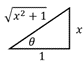
\includegraphics{images/trigsuba8.png}
    \end{figure}

    \(\tan{\theta}=x\\
    dx=\sec^2{\theta}\,d\theta\)

    \(\int \frac{\sqrt{\tan^2{\theta}+1}}{\tan{\theta}}\sec^2{\theta}\,d\theta\)

    \(\int \frac{\sec^3{\theta}}{\tan{\theta}}\,d\theta\)

    \(\int \frac{\sec{\theta}(\tan^2{\theta}+1)}{\tan{\theta}}\,d\theta\)

    \(\int \frac{\sec{\theta}\tan^2{\theta}+\sec{\theta}}{\tan{\theta}}\,d\theta\)

    \(\int \sec{\theta}\tan{\theta}\,d\theta+\int \frac{\sec{\theta}}{\tan{\theta}}\,d\theta\)

    \(\int \sec{\theta}\tan{\theta}\,d\theta+\int \frac{1}{\cos{\theta}}\times \frac{\cos{\theta}}{\sin{\theta}}\,d\theta=\int \sec{\theta}\tan{\theta}\,d\theta+\int \csc{\theta}\,d\theta\)

    To integrate \(\csc{\theta}\), multiply by \(\frac{\csc{\theta}-\cot{\theta}}{\csc{\theta}-\cot{\theta}}\):

    \(\int \sec{\theta}\tan{\theta}\,d\theta+\int \frac{\csc^2{\theta}-\csc{\theta}\cot{\theta}}{\csc{\theta}-\cot{\theta}}\,d\theta\)

    \(=\sec{\theta}+\ln{|\csc{\theta}-\cot{\theta}|}+c\)

    From the original triangle,

    \(\sec{\theta}=\frac{1}{\cos{\theta}}=\sqrt{x^2+1}, \csc{\theta}=\frac{1}{\sin{\theta}}=\frac{\sqrt{x^2+1}}{x}, \cot{\theta}=\frac{1}{\tan{\theta}}=\frac{1}{x}\)

    So the answer is:

    \(\int \frac{\sqrt{x^2+1}}{x}\,dx=\sqrt{x^2+1}+\ln{|\frac{\sqrt{x^2+1}-1}{x}|}+c\)

    \item 
    \(\int \frac{\sqrt{1-x^2}}{x}\,dx\)
    \begin{figure}[h]
        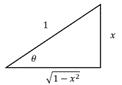
\includegraphics{images/trigsuba9.png}
    \end{figure}

    \(x=\sin{\theta}\\
    dx=\cos{\theta}\,d\theta\)

    \(\int \frac{\sqrt{1-\sin^2{\theta}}}{\sin{\theta}}\cos{\theta}\,d\theta\)

    \(\int \frac{\sqrt{\cos^2{\theta}}}{\sin{\theta}}\cos{\theta}\,d\theta\)

    \(\int \frac{\cos^2{\theta}}{\sin{\theta}}\,d\theta=\int \frac{1-\sin^2{\theta}}{\sin{\theta}}\,d\theta\)

    \(\int (\frac{1}{\sin{\theta}}-\sin{\theta})\,d\theta=\int (\csc{\theta}-\sin{\theta})\,d\theta\)

    To integrate \(\csc{\theta}\), multiply by \(\frac{\csc{\theta}-\cot{\theta}}{\csc{\theta}-\cot{\theta}}\):

    \(\int (\frac{\csc^2{\theta}-\csc{\theta}\cot{\theta}}{\csc{\theta}-\cot{\theta}}-\sin{\theta})\,d\theta\)

    \(\ln{|\csc{\theta}-\cot{\theta}|+\cos{\theta}}+c\)

    From the original triangle:

    \(\csc{\theta}=\frac{1}{\sin{\theta}}=\frac{1}{x}, \cot{\theta}=\frac{1}{\tan{\theta}}=\frac{\sqrt{1-x^2}}{x}, \cos{\theta}=\sqrt{1-x^2}\)

    So the integral is:

    \(\int \frac{\sqrt{1-x^2}}{x}\,dx=\ln{|\frac{1-\sqrt{1-x^2}}{x}|}+\sqrt{1-x^2}+c\)

    \item 
    \(\int \frac{(x^2-1)^{\frac{3}{2}}}{x}\,dx\)
    \begin{figure}[h]
        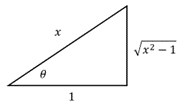
\includegraphics{images/trigsuba10.png}
    \end{figure}

    \(\cos{\theta}=\frac{1}{x}\\
    x=\sec{\theta}\\
    dx=\sec{\theta}\tan{\theta}\,d\theta\)

    \(\int \frac{(\sec^2{\theta}-1)^{\frac{3}{2}}}{\sec{\theta}}\sec{\theta}\tan{\theta}\,d\theta\)

    \(\int (\tan^2{\theta})^{\frac{3}{2}}\tan{\theta}\,d\theta\)

    \(\int \tan^4{\theta}\,d\theta\)

    \(\int \tan^2{\theta}(\sec^2{\theta}-1)\,d\theta\)

    \(\int (\tan^2{\theta}\sec^2{\theta}-\tan^2{\theta})\,d\theta\)

    \(\int (\tan^2{\theta}\sec^2{\theta}-\tan^2{\theta})\,d\theta\)

    \(\int \tan^2{\theta}\sec^2{\theta}-\int (\sec^2{\theta}-1)\,d\theta\)

    For the first part, use the substitution \(u=\tan{\theta}\), meaning \(du=\sec^2{\theta}\).

    \(\int u^2\,du=\frac{u^3}{3}=\frac{\tan^3{\theta}}{3}\)

    So the integral is:

    \(\frac{\tan^3{\theta}}{3}-\tan{\theta}+\theta+c\)

    From the original triangle, \(\tan{\theta}=\sqrt{x^2-1}, \theta=\cos^{-1}{\frac{1}{x}}\)

    \(\int \frac{(x^2-1)^{\frac{3}{2}}}{x}\,dx=\frac{(x^2-1)^{\frac{3}{2}}}{3}-\sqrt{x^2-1}+\cos^{-1}{(\frac{1}{x})}+c\)

    \item 
    \(\int \cos{x}\sqrt{9+25\sin^2{x}}\,dx\)
    \begin{figure}[h]
        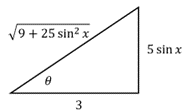
\includegraphics{images/trigsuba11.png}
    \end{figure}

    \(\tan{\theta}=\frac{5\sin{x}}{3}\\
    \sin{x}=\frac{3}{5}\tan{\theta}\\
    \cos{x}\,dx=\frac{3}{5}\sec^2{\theta}\,d\theta\)

    \(\int \sqrt{9+25(\frac{3}{5}\tan{\theta})^2}\frac{3}{5}\sec^2{\theta}\,d\theta=\frac{3}{5}\int \sqrt{9+9\tan^2{\theta}}\sec^2{\theta}\,d\theta\)

    \(\frac{3}{5}\int \sqrt{9(1+\tan^2{\theta})}\sec^2{\theta}\,d\theta=\frac{3}{5}\int 3\sec{\theta}\sec^2{\theta}\,d\theta\)

    \(\frac{9}{5}\int \sec{\theta}\sec^2{\theta}\,d\theta\)

    Using the DI method:

    \begin{tabular}{ c c c }
       & D & I \\ 
     +  & $\sec{\theta}$ &$\sec^2{\theta}$ \\  
     - & $\sec{\theta}\tan{\theta}$ & $\tan{\theta}$\\ 
    \end{tabular}

    Since we can easily integrate the product of the second row, we stop there:

    \(\frac{9}{5}\int \sec{\theta}\sec^2{\theta}\,d\theta=\frac{9}{5}(\sec{\theta}\tan{\theta}-\int \sec{\theta}\tan^2{\theta}\,d\theta)\)

    Focusing on the second part:

    \(\int \sec{\theta}\tan^2{\theta}\,d\theta=\int \sec{\theta}(\sec^2{\theta}-1)\,d\theta=\int \sec^3{\theta}\,d\theta -\int \sec{\theta}\,d\theta\)

    Substituting back:

    \(\frac{9}{5}\int \sec^3{\theta}\,d\theta=\frac{9}{5}(\sec{\theta}\tan{\theta}-\int \sec^3{\theta}\,d\theta +\int \sec{\theta}\,d\theta))\)

    We can move part of the equation to rearrange to this:

    \(\frac{18}{5}\int \sec^3{\theta}\,d\theta=\frac{9}{5}(\sec{\theta}\tan{\theta} +\int \sec{\theta}\,d\theta)\)

    \(\frac{9}{5}\int \sec^3{\theta}\,d\theta=\frac{9}{10}\sec{\theta}\tan{\theta} +\frac{9}{10}\int \sec{\theta}\,d\theta\)

    To integrate \(\sec{\theta}\), we multiply by \(\frac{\sec{\theta}+\tan{\theta}}{\sec{\theta}+\tan{\theta}}\)

    \(\int \sec{\theta}\,d\theta=\int \frac{\sec^2{\theta}+\sec{\theta}\tan{\theta}}{\sec{\theta}+\tan{\theta}}\,d\theta=\ln{|\sec{\theta}+\tan{\theta}|}+c\)

    Giving us:

    \(\frac{9}{5}\int \sec^3{\theta}\,d\theta=\frac{9}{10}\sec{\theta}\tan{\theta}+\frac{9}{10}\ln{|\sec{\theta}+\tan{\theta}|}+c\)

    From the original triangle, \(\sec{\theta}=\frac{1}{\cos{\theta}}=\frac{\sqrt{9+25\sin^2{x}}}{3}, \tan{\theta}=\frac{5\sin{x}}{3}\)

    Substituting into the integral to get the solution:

    \(\int \cos{x}\sqrt{9+25\sin^2{x}}\,dx=\frac{9}{10}\frac{\sqrt{9+25\sin^2{x}}}{3}\times \frac{5\sin{x}}{3}+\frac{9}{10}\ln{|\frac{\sqrt{9+25\sin^2{x}}}{3}+\frac{5\sin{x}}{3}|+c}\)

    \(=\frac{\sin{x}\sqrt{9+25\sin^2{x}}}{2}+\frac{9}{10}\ln{|\frac{\sqrt{9+25\sin^2{x}}}{3}+\frac{5\sin{x}}{3}|+c}\)
    \pagebreak
    \item 2022 Scholarship exam
    
    Show that \(\int \frac{1}{\sqrt{1+x^2}}\,dx=\ln{|\sqrt{1+x^2}+x|}+c\)
    \begin{figure}[h]
        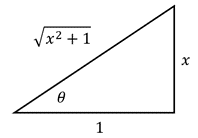
\includegraphics{images/trigsuba12.png}
    \end{figure}

    \(\tan{\theta}=x\\
    dx=\sec^2{\theta}\,d\theta\)

    \(\int \frac{1}{\sqrt{1+\tan^2{\theta}}}\sec^2{\theta}\,d\theta=\int \frac{1}{\sqrt{\sec^2{\theta}}}\sec^2{\theta}\,d\theta\)

    \(=\int \sec{\theta}\,d\theta\)

    To integrate \(\sec{\theta}\), we multiply by \(\frac{\sec{\theta}+\tan{\theta}}{\sec{\theta}+\tan{\theta}}\)

    \(\int \sec{\theta}\,d\theta=\int \frac{\sec^2{\theta}+\sec{\theta}\tan{\theta}}{\sec{\theta}+\tan{\theta}}\,d\theta=\ln{|\sec{\theta}+\tan{\theta}|}+c\)

    From the original triangle, \(\sec{\theta}=\frac{1}{\cos{\theta}}=\sqrt{x^1+1}, \tan{\theta}=x\)

    Therefore, \(\int \frac{1}{\sqrt{1+x^2}}\,dx=\ln{|\sqrt{x^2+1}+x|}+c\), as required.
    
\end{enumerate}


\pagebreak


\end{document}